\documentclass[12pt,a4paper]{report}
\usepackage[utf8]{inputenc}
\usepackage{amsmath}
\usepackage{amsfonts}
\usepackage{amssymb}
\usepackage{graphicx, neuralnetwork,tikz}
\usepackage{float}
\usetikzlibrary{positioning}
\input defs.tex
%\usepackage[style=numeric]{biblatex}
%\bibliographystyle{alpha}
\usepackage{url}
\graphicspath{ {./figures/} }
\usepackage{cite}


\tikzstyle{process} = [rectangle, minimum width=3cm, minimum height=1cm, text centered, draw=black]
\tikzstyle{arrow} = [thick,->,>=stealth]

\tikzstyle{state}=[shape=circle,draw=blue!30,fill=blue!10]
\tikzstyle{observation}=[shape=rectangle,draw=orange!30,fill=orange!10]
\tikzstyle{lightedge}=[<-, dashed]
\tikzstyle{mainstate}=[state, thick]
\tikzstyle{mainedge}=[<-, thick]
\tikzstyle{block} = [draw,rectangle,thick,minimum height=2em,minimum width=2em]
\tikzstyle{sum} = [draw,circle,inner sep=0mm,minimum size=2mm]
\tikzstyle{connector} = [->,thick]
\tikzstyle{line} = [thick]
\tikzstyle{branch} = [circle,inner sep=0pt,minimum size=1mm,fill=black,draw=black]
\tikzstyle{guide} = []
\tikzstyle{snakeline} = [connector, decorate, decoration={pre length=0.2cm,
                         post length=0.2cm, snake, amplitude=.4mm,
                         segment length=2mm},thick, magenta, ->]




\title{Neural Network Based Sequence Detection over Molecular Mommunication Channels}
\author{Peter Hartig}
%Remove this penaltiy if hyphenation is okay. 
%\hyphenpenalty=10000

\begin{document}
\maketitle

\begin{abstract}
Estimation of the probability distribution function characterizing a communication channel is investigated. In this work, pilot symbol sequences are used to train a neural network to estimate unknown channel probability distribution functions. The estimated function is then evaluated as a metric for the Viterbi algorithm. In particular, the detection performance is investigated for channels relevant to the molecular communications domain. A proposal is then made to reduce the complexity of the resulting detection scheme using a second supervised learning method. The neural network based estimation is tested in simulations and shown to be effective in detection for (DESCRIBE CHANNELS) channels. 
\end{abstract}

\newpage
\tableofcontents
\newpage
\section{Notation}
This section details the notation is throughout this work.
$p(x)$ is the probability of an event $x$.
$p(x|y)$ is the conditional probability of $x$ given $y$.
$E[x]$ is the expected value of a random variable .
$x \sim \mathcal{N}(0,1)$ denotes a random variable $x$ whose probability distribution is Gaussian with mean 0 and variance 1. 

Vectors are denoted by bold font lower-case letters ($\mathbf{x}$) and are assumed column vectors.
The vector $\mathbf{x}_{\mathrm{i}}^{\mathrm{j}}$ denotes a vector containing the elements i through j of $\mathbf{x}$. Sets are denoted using upper-case calligraphic letters ($\mathcal{A}$) and the cardinality of a set $\mathcal{A}$ is denoted by $|\mathcal{A}|$.
$\underset{x}{\text{argmin}} \; f(x)$ is the value of variable $x$ which minimizes the function $f(x)$.

\section{Introduction}

The general communication channel is equivalent to a conditional probability distribution function (pdf). The channel pdf $p(\mathbf{x}|\mathbf{y})$ takes into account the (potentially random) channel though which the transmitted information $\mathbf{x}$ passes to reach a receiver as the information $\mathbf{y}$ \cite[Ch.~7]{cover2012elements}. Selecting the most probable transmitted information sequence based on the received information sequence is known as maximum a posteriori (MAP) sequence estimation. In general, sub-optimal solutions to this estimation problem do not require perfect knowledge of the pdf $p(\mathbf{x}|\mathbf{y})$ and may be used when the true $p(\mathbf{x}|\mathbf{y})$ is unknown or impractical to obtain.

\par
Some communication contexts, including wireless, have successfully used "pilot" symbol-streams to estimate the pdf $p(\mathbf{x}|\mathbf{y})$ \cite{van1995channel}. The receiver is informed of a symbol sequence prior to receiving that same sequence sent through the channel. The receiver may then compare the received signal with the known ground truth to estimate the channel $p(\mathbf{x}|\mathbf{y})$.
The use of pilot sequences typically relies on a pre-selected channel model whose parameters are determined using the pilot sequence. For example, if the channel is assumed to be a noiseless, linear and time-invariant (LTI) system, the pilot sequences may be used to find the exact impulse response of the channel as will be seen in this work. In some cases, however, a precise channel model may not be available. This work investigates the parameterization of a very general channel model for $p(\mathbf{x}|\mathbf{y})$ using a neural network. In previous work, neural network based estimation of the channel has shown to be an effective method for detection with incomplete channel information for linear, time-invariant channels \cite{shlezinger2019viterbinet} \cite{shlezinger2020datadriven}.
 Extending on this, we look to estimate $p(\mathbf{x}|\mathbf{y})$ for channels in the molecular communication domain.
 We also look to exploit any redundancy in the pdf $p(\mathbf{x}|\mathbf{y})$ in order to reduce the complexity of the resulting detection algorithm.
\par
Molecular communication channels can be difficult to characterize due to their non-linear and random components that may or may not depend upon the transmitted information. As a result, molecular communication channels are good candidates for testing this estimation technique. For a thorough review and mathematical formulation of molecular communication channels and their applications see \cite{jamali2019channel}. 

\par

\section{System Model}

A system model is now developed as a consistent communication framework to be used in the remainder.
\par
We consider a point to point communication system as in Figure \ref{fig:model} with a transmitter sending a sequence of information $\mathbf{x}$ over a channel. At the receiver, the sequence  $\mathbf{y}$ is detected. 
The elements of $\mathbf{x}$ are chosen from a finite symbol alphabet $\mathcal{A}$ such that $x[\text{k}] \in \mathcal{A}$.

\begin{figure}[H]
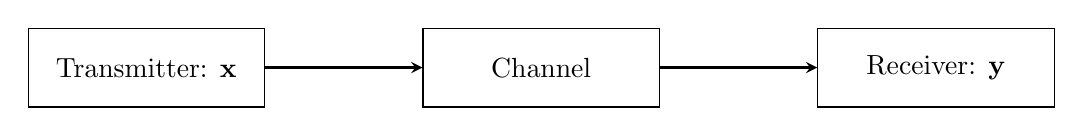
\begin{tikzpicture}[node distance=2cm]
\node (transmitter) [process] {Transmitter: $\mathbf{x}$};
\node (channel) [process, right = of transmitter] {Channel};
\node (receiver) [process, right = of channel] {Receiver: $\mathbf{y}$};
\draw [arrow] (transmitter) -- (channel);
\draw [arrow] (channel) -- (receiver);
\end{tikzpicture}
\caption{The point to point communication system.}
\label{fig:model}
\end{figure}

The components of the vector $\mathbf{y}$ are described by 
\begin{equation*}
y[\text{k}] = f_{\text{k}}(\mathbf{x}) + n[\text{k}],
\end{equation*}
with independent $n[\text{k}]\sim \mathcal{N}(0,1).$
Allowing for $f_{\text{k}}()$ to be a general and potentially random function, each received symbol $y[\text{k}]$ is potentially a function of all input information $\mathbf{x}$.

By assuming all $n[\text{k}]$ to be independent, an orthogonal filtering of the modulated information $\mathbf{x}$ at the receiver is implied. We define the signal to noise ratio (SNR) at the receiver as 

\begin{equation*}
\text{SNR} = \frac{E\{|x[\text{k}]|^2\}}{\sigma^2}.
\end{equation*}
	We now consider specific cases for the function $f_{\text{k}}()$ that will later be used in describing the detection methods. 
	\par
In the first communication channel $f_{\text{k}}(\mathbf{x}) + n[\text{k}]$ considered, each $y[\text{k}]$ is a causal, linear, and time-invariant (LTI) combination of the transmitted sequence $[x[\text{k}], x[\text{k}-1]... x[\text{K}-\text{L}+1]]$ weighted by coefficients $[a[0], a[1].. . [\text{L}-1]]$. 
\begin{equation*}
y[k] = \sum_{\mathrm{\text{l}=0}}^{\mathrm{\text{L}-1}} a[\text{l}]x[\text{k}-\text{l}].
\end{equation*}

\par 
We also consider the case in which the received output from an arbitrary communication channel is quantized giving
\begin{equation*}
y[\text{k}] = \text{Quant}(f_{\text{k}}(\mathbf{x}) + n[\text{k}])
\end{equation*}
 with
\[\text{Quant}(x) = 
\begin{cases}
\text{sign}(x)\text{floor}(\frac{x}{\text{step size}})& \text{lower saturation level} \leq x \leq \text{upper saturation level}\\
\text{upper saturation level} & x \geq \text{upper saturation level}\\
\text{lower saturation level} & x \leq \text{lower saturation level}
\end{cases}
\]
 for 
 \begin{equation*}
  \text{step size} =\text{floor}\left(\frac{|\text{upper saturation level}- \text{lower saturation level}|}{\text{\# Quantization levels}}\right).
 \end{equation*} A quantizer with 20 quantization levels and lower/upper saturation levels -5/+5 respectively is shown in Figure \ref{fig:Quantized Overlay}.
 
 \begin{figure}[H]
\centering
	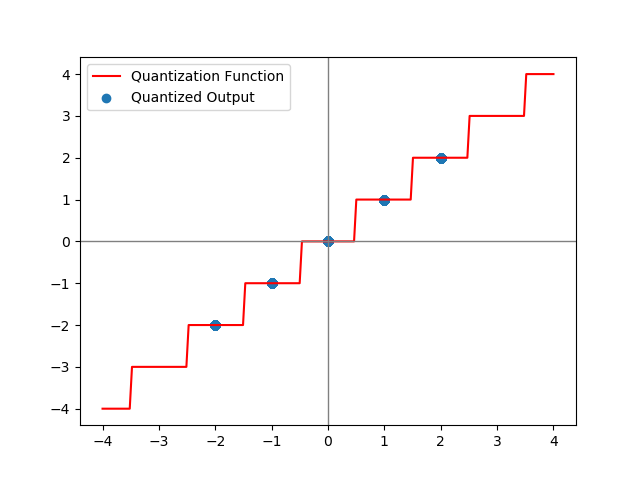
\includegraphics[width=10cm,height = 10cm]{system_model/quantizer_overlay}
			  \caption{Quantizer with 20 quantization levels, lower saturation levels  $= -5$ and upper saturation levels  $= +5$}.
	  \label{fig:Quantized Overlay}
\end{figure}
 
\section{Background}
The following section first introduces the optimization problem used in the remainder of this work. An efficient implementation for solving the optimization problem is then introduced. With this foundation in place, the data-driven, neural network based estimator is then incorporated into the optimization algorithm. 
Extending on the neural network based detector, a method to further reduce the algorithm complexity is then considered. Lastly, a linear equalizer is derived to be used as a reference in the simulation results. 
\subsection{MLSE and the Viterbi Algorithm}
Rather than considering only the transmitted symbols $\mathbf{x}$  for the MAP problem described above, instead consider a system in which a sequence $\mathbf{y}$ is received from a channel which may take on a set of states $\{s_1, s_2... s_{\text{L}}\} = \mathcal{S}$. With knowledge of the potential states $\{s_1, s_2... s_{\text{L}}\}$ but not the sequence of realized states $[s[1], s[2]... s[\text{N}]]$ corresponding to $[y[1], y[2]... y[\text{N}]]$, the MAP problem is restated as

\begin{equation*}
\underset{\mathbf{s}\in\mathcal{S}^N}{\text{argmax}} \; p(\mathbf{s}|\mathbf{y}).
\end{equation*} 

Using Bayes' theorem, we can equivalently use 
\begin{equation*}
p(\mathbf{s}|\mathbf{y}) = 
\frac
{p(\mathbf{y}|\mathbf{s})p(\mathbf{s})}
{p(\mathbf{y})}.
\end{equation*}
The term $p(\mathbf{y})$ is independent of $\mathbf{s}$ so it is removed without effect. The resulting optimization problem
\begin{equation}\label{opt_problem}
\underset{\mathbf{s}\in\mathcal{S}^N}{\text{argmax}}\; p(\mathbf{y}|\mathbf{s})p(\mathbf{s})
\end{equation}
will be used in the remainder.
Noting that the size of the search space $|\mathcal{S}^N|$ grows exponentially in $N$, the number of received symbols, a method for reducing the search complexity is now introduced. 
\par
For the LTI communication channel described in the system model section, each state $s_i \in \{s_1, s_2... s_{\text{L}}\}$ represents a possible transmitted sequence $[x[\mathrm{i-L+1}]...x[\mathrm{i}]]$  and $p(\mathbf{x})=p(\mathbf{s})$. If all symbols in $\mathcal{A}$ are selected with equal probability, as is commonly assumed to maximize information entropy for finite $|\mathcal{A}|$, the term $p(\mathbf{x})$ can be removed from problem \ref{opt_problem} without effect. 
For this channel,
\begin{gather*}
\underset{\mathbf{s}\in\mathcal{S}^N}{\text{argmax}} \; p(\mathbf{y}|\mathbf{s})p(\mathbf{s})=
\underset{\mathbf{s}\in\mathcal{S}^N}{\text{argmin}} \; \sum_{\mathrm{i=1}}^{\mathrm{N}} -\text{log}(p(y[\mathrm{i}]|s[\mathrm{i}]) p(s[\mathrm{i}]|s[\mathrm{i-1}]))=\\
\underset{\mathbf{x}\in\mathcal{A}^N}{\text{argmin}} \; \sum_{\mathrm{i=1}}^{\mathrm{N}} -\text{log}(p(y[\mathrm{i}]|\left[x[\mathrm{i-L+1}]...x[\mathrm{i}]\right]) p(\left[x[\mathrm{i-L+1}]...x[\mathrm{i}]\right]|\left[x[\mathrm{i-L}]...x[\mathrm{i-1}]\right]))
\end{gather*}
in which individual terms of the sums are statistically independent. The optimization problem is equivalently
  represented by a graph with the L states $\{s_1, s_2... s_{\text{L}}\}$ repeated N times and all states in time k, $s_{\text{i}}[\text{k}], \; i = 1... \;L$ connected to all states in time k$+1$, $s_{\text{i}}[\text{k+1}], \; i = 1... \;L$ 
   by an edge weighted with
\begin{equation*}
-\text{log}(p(y[\text{k}+1]|s_{\text{i}}[\text{k+1}])p(s_{\text{i}}[\text{k+1}]|s_{\text{j}}[\text{k}])).
\end{equation*}   
This is illustrated in the following example. 
   \par
   Consider the communication system with $\mathcal{A}=\{0, 1\}$ and received symbols 
   \begin{equation*}
y[\text{k}] =  a[\text{0}]x[\text{k}] + a[\text{1}]x[\text{k}-1] + n[\text{k}],
\end{equation*}
with $n[\text{k}] \sim \mathcal{N}(0,1)$.
The resulting state graph (or trellis) is depicted in Figure \ref{fig:trellis}. 
Again assuming equiprobable 
$x[\text{k}] \in \mathcal{A}$, the value of $p(s_{\text{j}}[\text{k+1}]|s_{\text{i}}[\text{k}])$ for connected states $s_{\text{j}}[\text{k+1}]$ and $s_{\text{j}}[\text{k}]$ is  0, if the channel memory represented by $s_{\text{j}}[\text{k+1}]$ and $s_{\text{j}}[\text{k}]$ contradicts. $p(s_{\text{j}}[\text{k+1}]|s_{\text{i}}[\text{k}])$  is some constant c ($0<$ c $\leq1$) if these states agree on the channel memory. For clarity, all edges for which $p(s_{\text{j}}[\text{k+1}]|s_{\text{i}}[\text{k}])=0$ have been removed in Figure \ref{fig:trellis}. Therefore the edges into state $s_{\text{i}}[\text{k+1}]$ are weighted by
$-\text{log}(p(y[\text{k}+1]|s_{\text{j}}[\text{k+1}])$. The solution to problem \ref{opt_problem} corresponds to the minimum cost path through all N sets of states which can be found using the Viteribi algorithm. 
\\

    \noindent\rule[16pt]{\textwidth}{0.6pt}
	Viterbi Algorithm: (TODO: Decide if this is clear enough)

    \noindent\rule[10pt]{\textwidth}{0.4pt}
    {\footnotesize
    \begin{tabbing}
        {\bf given} $p(y[\text{k}]|s_{\text{i}}[\text{k}])$, $p(s_{\text{l}}[\text{k+1}]|s_{\text{j}}[\text{k}]) \; \forall  \; \text{k} \in {1..N}$ and $ \forall \; \text{j} \in {1..L}$. \\*[\smallskipamount]
        {\textbf{for}  $\text{k} = 1... N $} \\
         \qquad \= {\textbf{for} $\text{i} = 1... L$}\\
        \qquad \qquad \= \textbf{Let} $\text{cost}_{\text{i}}[\text{k}] = \underset{\text{j} \in \{1...L\}} {\text{argmin}}\left( \text{cost}_{\text{j}}[\text{k-1}]
        -\text{log}(p(y[\text{k}]|s_{\text{i}}[\text{k}])p(s_{\text{i}}[\text{k}]|s_{\text{j}}[\text{k-1}]))
        \right)$ \\
        {\bf return} detected transmission $\hat{\mathbf{x}}$ corresponding to trellis path of $\underset{\text{i} \in \{1...L\}} {\text{argmin}} \; \text{cost}_{i}[\text{N}] $
    \end{tabbing}}
    \noindent\rule[10pt]{\textwidth}{0.4pt}



\begin{figure}[H]
\begin{center}
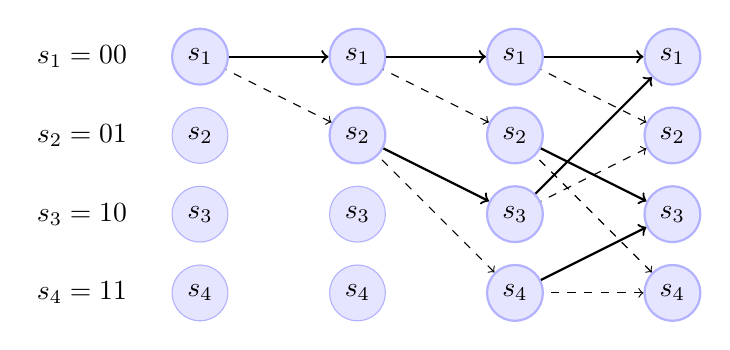
\begin{tikzpicture}[]
% 1st column
\node               at (-1.5,5) {$s_1=00$};
\node               at (-1.5,4) {$s_2=01$};
\node               at (-1.5,3) {$s_3=10$};
\node               at (-1.5,2) {$s_4=11$};
\node[mainstate] (s1_1) at (0,5) {$s_1$};
\node[state] (s2_1) at (0,4) {$s_2$};
\node[state] (s3_1) at (0,3) {$s_3$};
\node[state] (s4_1) at (0,2) {$s_4$};
%\node at (0,1) {Node1};
% 2nd column
\node[mainstate] (s1_2) at (2,5) {$s_1$}
    edge[mainedge] (s1_1);
\node[mainstate] (s2_2) at (2,4) {$s_2$}
     edge[lightedge] (s1_1);

\node[state] (s3_2) at (2,3) {$s_3$};

\node[state] (s4_2) at (2,2) {$s_4$};

%\node at (2,1) {Node2};
% 3rd column
%\node               at (4,6) {$t=2$};
\node[mainstate] (s1_3) at (4,5) {$s_1$}
    edge[mainedge]  (s1_2);

\node[mainstate] (s2_3) at (4,4) {$s_2$}
    edge[lightedge] (s1_2);

\node[mainstate] (s3_3) at (4,3) {$s_3$}
    edge[mainedge] (s2_2);    
\node[mainstate] (s4_3) at (4,2) {$s_4$}
    edge[lightedge] (s2_2);
%\node at (4,1) {Node3};
% 4th column
%\node               at (6,6) {$t=3$};
\node[mainstate] (s1_4) at (6,5) {$s_1$}
    edge[mainedge]  (s1_3)
    edge[mainedge]  (s3_3);
\node[mainstate] (s2_4) at (6,4) {$s_2$}
    edge[lightedge] (s1_3)
    edge[lightedge] (s3_3);
\node[mainstate] (s3_4) at (6,3) {$s_3$}
    edge[mainedge] (s2_3)
    edge[mainedge] (s4_3);
\node[mainstate] (s4_4) at (6,2) {$s_4$}
    edge[lightedge] (s2_3)
    edge[lightedge] (s4_3);
%\node at (6,1) {Node4};

\end{tikzpicture}
	\end{center}
	\caption{MLSE decoding for $\mathcal{A}=\{0,1\}$ and $L=2$. Each state $s_1 ... \; s_4$ represents a possible
	$\left[x[\mathrm{i-L+1}]...x[\mathrm{i}]\right]$.}
	\label{fig:trellis}
\end{figure}

Note that the Viterbi algorithm is \emph{linearly} complex in the length of the sequence $\mathbf{s}$ ($N$ in the algorithm above) but \emph{exponentially} complex in the number of channel states $|\mathcal{S}|$. 
\par
The above model allows channels whose state is based upon transmitted symbols to be represented using a trellis, such as the LTI channel. This graph based model can also generalize to represent channels with certain kinds randomness that is \emph{independent} of the transmitted symbols. In this case, the model is constrained to channels whose state satisfies the property
\begin{equation*}
p(\mathbf{s}) = p(s[\text{N}]|s[\text{N-1}]) p(s[\text{N-1}]|s[\text{N-2}])... p(s[\text{2}]|s[\text{1}])p(s[\text{1}]),
\end{equation*}
which implies the Markov property

\begin{equation*}
p(s[\text{k}]|\left[s[\mathrm{1}]...s[\mathrm{k-1}]\right],\left[s[\mathrm{k+1}]...s[\mathrm{N}]\right]) = p(s[\text{k}]|s[\text{k-1}]).
\end{equation*}

An example of such a channel is the same LTI system described above, but with a two-state noise floor satisfying the Markov property (TODO simulate and if results then detail model and reference to results)
\par
Lastly, this model can also represent the case in which a channel state $s[k]$ does not uniquely identify a symbol $x[k]$ that was transmitted in the corresponding time index. While this case requires additional tools to ultimately arrive at a unique transmit sequence $\mathbf{x}$ it may also reduce the complexity of the corresponding Viterbi algorithm. This case will be considered in more detail later in this work.
\par
In the remainder of this work, we consider the case in which the  channel state is determined entirely by $\left[x[\mathrm{i-L+1}]...x[\mathrm{i}]\right]$, as was the case for the basic LTI channel (Remove if results above work). 

\subsection{ViterbiNet}

Despite the complexity reduction of the Viterbi Algorithm for MAP detection, weighting the edges of the graph requires knowledge of the channel probability distribution $p(y[\mathrm{k}]|s[\mathrm{k}])$. Rather than estimate this function directly, we use Bayes' theorem and instead estimate the individual terms of
\begin{equation*}
p(y[\mathrm{k}]|s_{\text{i}}[\text{k}]) = 
\frac
{p(s_{\text{i}}[\text{k}]|y[\mathrm{k}])p(y[\mathrm{k}])}
{p(s_{\text{i}}[\text{k}])}.
\end{equation*}

\begin{itemize}
\item $p(s_{\text{i}}[\text{k}]|y[\mathrm{k}])$: 
For a channel with finite states $\{s_1, s_2,.. s_{\text{L}}\}$, this probability mass function can be estimated using a neural network for classification. Each training data pair includes a single received pilot symbol $y[\text{k}]$ (the network input ) and the probability of being in a state
$s_{\text{i}}[\text{k}] \sim \left[x[\mathrm{i-L+1}]...x[\mathrm{i}]\right]$ (the network output). The true state is known for pilot symbols. By using using a network architecture with a number of outputs corresponding to the number of channel states, the trained network will output the desired $p(s_{\text{i}}[\text{k}]|y[\text{k}])$ for all $s_{\mathrm{i}} \in \textit{\cal{S}}$. Figure \ref{nn} depicts the neural network for a channel with four states. The shown network has a total of edges (model parameters) to be optimized during training. For a detailed review of classification using neural networks, see \cite[Ch.~5]{Goodfellow-et-al-2016}.

	\begin{figure}[H]
	\centering
		\begin{neuralnetwork}[height=4.5, nodespacing=20mm, layerspacing=24mm]
		\newcommand{\x}[2]{$y[\text{k}]$}
		\newcommand{\y}[2]{$p(s_{#2}[\text{k}]|y[\text{k}])$}
		\newcommand{\hfirst}[2]{ $h^{(1)}_#2$}
		\newcommand{\hsecond}[2]{ $h^{(2)}_#2$}
		\newcommand{\hthird}[2]{$h^{(3)}_#2$}
		\newcommand{\hfourth}[2]{$h^{(4)}_#2$}
		\inputlayer[count=1, bias=false, title=Received\\, text=\x]
		\hiddenlayer[count=2, bias=false, title=\\, text=\hthird] \linklayers
		\hiddenlayer[count=3, bias=false, title=\\, text=\hfourth] \linklayers
		\outputlayer[count=4, title=States\\, text=\y] \linklayers
	    \end{neuralnetwork}
	    	  	  \caption{A fully-connect, feed-forward neural network architecture for classification of received symbols $y[\text{k}]$ into four channel states.}
\label{nn}
	\end{figure}

\item $p(y[\mathrm{k}]) = \sum_{s_{\mathrm{i}} \in \textit{$\mathcal{S}$}}p(s_{\mathrm{i}},y[\mathrm{i}])$: This term is found by marginalizing the joint probability of channel state $s_{\mathrm{i}}[\mathrm{k}]$ and received signal $y[\mathrm{k}]$ over all channel states $\mathcal{S}$. As $p(y[\mathrm{k}])$ is constant over all states in a given step of the Viterbi algorithm, it may be interpreted as a weighting factor for the cost of received symbol $y[\mathrm{k}]$ relative to other symbols $y[\mathrm{j}], \; j\neq k$. For example, if $y[\mathrm{k}]$ is received under improbable noise and channel state, this term would reduce the overall impact of $y[\mathrm{k}]$ on the final path chosen through the graph. In the case of equiprobable channel states without receiver noise $p(y[\mathrm{k}])$ would be constant and have no impact on the chosen path.
\par
This probability distribution function can be estimated using a so-called mixture-model. This requires pre-selecting the number of considered channel states and a parameterized model for receiver noise. The Expectation Maximization algorithm, detailed in \cite{ng2000cs229}, along with a set of channel output to train the model with, can be used to optimize this model. Unlike parameterizing the neural network this algorithm does not require labeled data. 
 (Figure \ref{fig:mm})
%\\
%
%    \noindent\rule[16pt]{\textwidth}{0.6pt}
%	Expectation Maximization Algorithm for Gaussian Mixture Model: (TODO Discuss how much derivation is needed here)
%
%    \noindent\rule[10pt]{\textwidth}{0.4pt}
%    {\footnotesize
%    \begin{tabbing}
%        {\bf given} $p(y_{\mathrm{i}}|x_{\mathrm{i-L+1}}^{\mathrm{i}}) \; \forall i \in {1..N}$ . \\*[\smallskipamount]
%        {\bf for $i = 1..N $} \\
%         \qquad \= {\bf for each state $s$ at time $i$}\\
%        \qquad \qquad \= 1.\ Let $\textit{survivor cost}_{s}  += \text{min}\{\text{incoming transition costs}\}$ \\
%%        \> 2.\ {\bf break if} $f(z) \leq \hat{f}_{\lambda}(z, x^{k})$. \\
%%        \> 3.\ Update $\lambda := \beta \lambda$. \\*[\smallskipamount]
%        {\bf return} Symbols corresponding to path of $\underset{s}{\text{argmin}} \; \textit{survivor cost}_{s} $
%    \end{tabbing}}
%    \noindent\rule[10pt]{\textwidth}{0.4pt}


%picture of MM
%	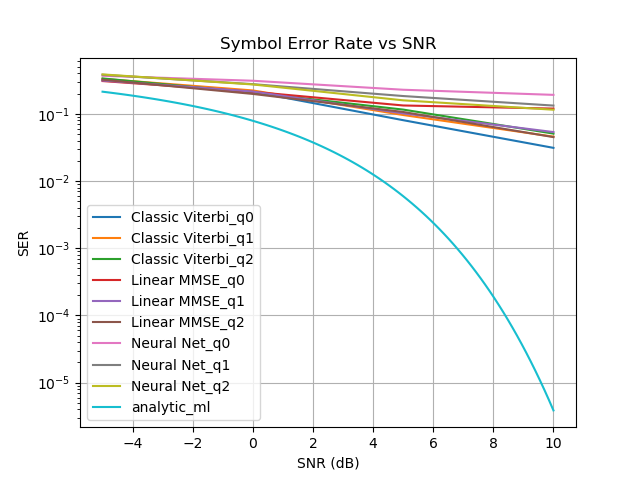
\includegraphics[width=\textwidth,height = 7cm]{results/quant_standard}

\begin{figure}[H]
\centering
	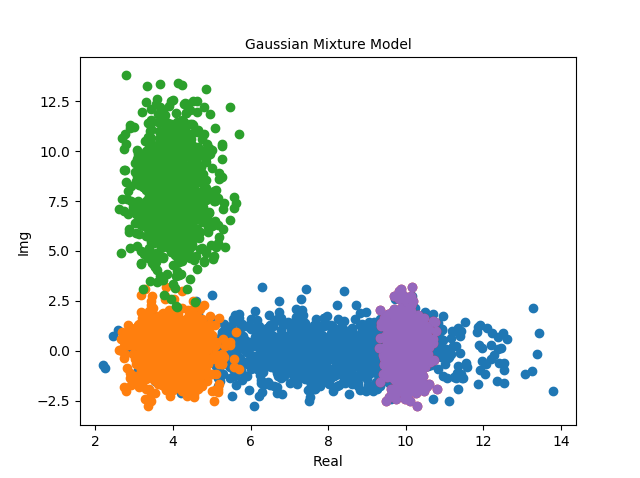
\includegraphics[width=\textwidth,height = 10cm]{system_model/mm}
	  	  \caption{A mixture of complex, Gaussian sources that can be estimate using the Expectation Maximization algorithm}
	  \label{fig:mm}
\end{figure}

\item $p(s[\text{k}])$: For the case in which each channel state is equiprobable, such as when $s_{\text{k}}$ corresponds to $\left[x[\mathrm{i-L+1}]...x[\mathrm{i}]\right] \in \mathcal{A}_{\mathrm{i-L+1}}^{\mathrm{i}}$, this term will not influence the final path and can be neglected.

\end{itemize}

Combining these terms and their impact on the original $p(y[\mathrm{k}]|s_{\text{i}}[\text{k}])$, each edge weight used in the Viterbi algorithm essentially gives the probability of simultaneously arriving at a state $s_{\text{i}}[\text{k}]$ conditioned on the previous state $s_{\text{i}}[\text{k-1}]$ and the probability of receiving $y[\mathrm{k}]$ based on the channel and noise. 
We now consider how a channel might be represented using the minimum number of states.

\subsection{A Reduced State ViterbiNet}
While the Viterbi Algorithm complexity scales exponentially in the number of states possible in each step of the algorithm, in some cases this complexity can be reduced without significant loss of detection performance. One well-established method to achieve this is by pre-filtering the incoming signal so as have a minimum-phase system representing the channel (TODO Cite). Such methods, however, are often dependent upon an estimate of the channel, again implying an assumed underlying channel model. In this section, we consider a method for this complexity reduction without pre-filtering the estimated channel.

There are two things to note here, first, this pre-filtering works for LTI channels but may not be possible for channels with non-linearities (such as molecular communication channels). Also note that even this minimum phase representation of the channel still has redundancy that could be reduced using this method. Finally, this pre-filtering assumes some sort of estimate and model of the channel that we are trying to abstract from in this work for generality. 


In the following, relevant example a channel is proposed whose states, as seen by the receiver, contain redundancy. One method for reducing the number of states based on this observed redundancy is then considered. 

Consider a received signal from an LTI communication channel
\begin{equation*}
y[k] = \sum_{\mathrm{l=1}}^{\mathrm{L}} a[l]x[k-l] + n[k], \; n[k]  \sim \mathcal{N}(0,1)
\end{equation*}

with  $\mathcal{A}=\{-1, 1\}$ and $n[k]  \sim \mathcal{N}(0,1)$.  

For $\mathbf{a} = [a[1]...a[5]]=[1, 0, .2, .2, .4]$ ($\|\mathbf{a}\|^2_2 = 1$), the received signal is shown in Figure \ref{fig:redundant_channel}. Desipite having channel memory L $=5$, there are fewer than the potential $|\mathcal{A}_{\mathrm{i-L+1}}^{\mathrm{i}}| =2^5$ clusters of received signals. This is due to the redundancy in the channel.  As one of the channel taps is 0, this will have no impact on the output seen at the receiver and thus 16 of the potential 32 states are removed. Further, as there are two taps of value 0.2 and $\mathcal{A}=\{-1, 1\}$, when $\left[x[k-2],x[k-3]\right] = [-1,1]$ and $\left[x[k-2],x[k-3]\right] = [1,-1]$ these map to the same output as seen by the receiver. 

%\begin{figure}[H]
%\centering
%	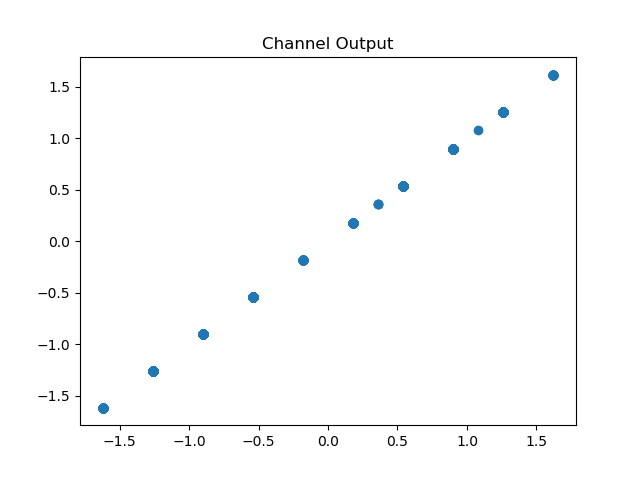
\includegraphics[width=10cm,height = 10cm]{system_model/channel_output}
%	  \label{fig:redundant_channel}
%	  	  \caption{LTI channel with state redundancy with high SNR}
%\end{figure}

\par
One data-driven approach to exploiting state redundancy is to cluster the observed states (receiver output) into a set of $k<|\mathcal{S}|$ clusters using training data. The k-Means algorithm is proposed as one such clustering method.
\\

    \noindent\rule[16pt]{\textwidth}{0.6pt}
k-Means Clustering Algorithm: A method for unsupervised classification

    \noindent\rule[10pt]{\textwidth}{0.4pt}
    {\footnotesize
    \begin{tabbing}
    {\bf given} initial location $L_c, \forall \;c  \in \{1..K\}$ of K centroids.\\
        {\textbf{for} Number of Iterations}.\\
         \qquad \= {\bf for each training data point $x_{\mathrm{i}}, \;\mathrm{i}  \in \{1..N\}$}\\
        \qquad \qquad \= 1.\ Label $x_i$ with the index c of the closest centroid using $\|x_{\mathrm{i}}- \text{L}_c\|^2_2$. \\
        \qquad \= {\bf for centroid $L_c, \forall \;c  \in \{1..K\}$}\\
                \qquad \qquad \= 1.\ Move $L_{\mathrm{c}}$ to the average location of all training points with label .c\\


%        \> 2.\ {\bf break if} $f(z) \leq \hat{f}_{\lambda}(z, x^{k})$. \\
%        \> 3.\ Update $\lambda := \beta \lambda$. \\*[\smallskipamount]
        {\bf return} Centroid locations.
    \end{tabbing}}
    \noindent\rule[10pt]{\textwidth}{0.4pt}
    

\par
An important implementation consideration for this clustering approach is now discussed. If the channel has memory $\text{L}>1$, at least some of the channels states represent different channel inputs as described previously. If states with contradicting transmission memory are clustered during the state reduction, the choice for the transmitted symbol is unclear. To accommodate this scenario, a majority rule decision is made, based on the final state path chosen by the Viterbi algorithm. During the clustering, the fraction of training samples from the original states labeled in each reduced state are recorded to give the likelihood of each symbol in the state memory. After finding the lowest cost path through the trellis, the probability of a symbol for each time index is found and the most likely is chosen. Note that this operation is \emph{not} exponentially complex in the memory length of the channel.

\par 
Clearly an appropriate number of clusters will influence the performance of the resulting decoder (Have figure showing this).

\subsection{Equalization benchmark}
The Linear Minimum Mean-Squared Error (LMMSE) equalizer derived below is used provide a linear equalization reference to the non-linearity of the proposed neural network based equalization .
\par
Given an estimate of channel memory length L, the convex and continuously differentiable optimization problem 

\begin{equation*}\label{mmse}
\underset{\mathbf{\mathbf{h}} \in \textit{$\mathcal{C}^{\text{L}}$}}{\text{argmin}} \;
 E[\|x-\mathbf{h}^T\mathbf{y}\|^2],
\end{equation*}\
minimizes the squared difference of the linearly detected symbol $\hat{x}= \mathbf{h}^T\mathbf{y}$ and true symbol $x$.
Using
\begin{equation*}\label{mmse}
\frac{\partial  E[\|x-\mathbf{h}^T\mathbf{y}\|^2]}{\partial \mathbf{h} } = 0
\end{equation*}
the optimal LMMSE equalizer is \cite{proakis1988introduction}
\begin{equation*}\label{mmse}
\mathbf{h} = E[\mathbf{R}_{yy}]^{-1}E[\mathbf{r}_{yx}].
\end{equation*}
$E[\mathbf{R}_{yy}]$ and $E[\mathbf{r}_{yx}]$ are estimated by
\begin{equation*}\label{mmse}
 E[\mathbf{R}_{yy}]= \frac{1}{\mathrm{N}}\sum_{\mathrm{i=1}}^{\mathrm{N}}
\mathbf{y^{\text{i}}_{\text{i-L+1}}}\mathbf{y^{\text{i}}_{\text{i-L+1}}}^H
 \end{equation*}
 and
\begin{equation*}\label{mmse}
E[\mathbf{r}_{yx}]= \frac{1}{\mathrm{N}}\sum_{\mathrm{i=1}}^{\mathrm{N}}
\mathbf{y^{\text{i}}_{\text{i-L+1}}}x_{\text{i}}
;
 \end{equation*}
 using the same training data as the neural network and mixture model. 
 
\par
One interesting note to make in comparing this equalizer with the neural network based equalizer is the amount of training data needed. In the case of the noiseless LTI system, a linear estimator for the channel requires only L training examples to form a deterministic system of equations and learn the channel perfectly. In contrast the neural network will generally have many edge weights and would therefore require more training data. The need for a larger training data set comes with the added potential to learn more complicated channels with the neural network than with the LMMSE equalizer.
 
\par
In the results below, the theoretical symbol error rate curve is also included as a reference.
For all of the tests below, an anti-podal BPSK scheme is simulated. The probability of a decision error for the memoryless AWGN channel with SNR 
\begin{equation*}\label{mmse}
E[\mathbf{r}_{yx}]= \frac{1}{\mathrm{N}}\sum_{\mathrm{i=1}}^{\mathrm{N}}
\mathbf{y^{\text{i}}_{\text{i-L+1}}}x_{\text{i}}.
 \end{equation*}

is \cite{proakis1988introduction} 

\begin{equation*}\label{mmse}
E[\mathbf{r}_{yx}]= \frac{1}{\mathrm{N}}\sum_{\mathrm{i=1}}^{\mathrm{N}}
\mathbf{y^{\text{i}}_{\text{i-L+1}}}x_{\text{i}}.
 \end{equation*}



\section{Results}

\subsection{Simulation Details}
The following simulations are performed using only real-valued transmit symbols, channels and noise. As a result, an SNR adjustment factor of 3dB has been used in order to align well-know results with other sources. 
\subsubsection{Implementation Details}
This section defines relevant information for implementation of the simulation used to generate the results below.
\begin{itemize}
\item \textbf{Neural Network}
The neural network used in this simulation was implemented using the PyTorch machine learning library. The network architecture and training parameters used are as follow:
\begin{itemize}
\item Architecture: 4 layers {1, 100 (Tanh activation), 50 (relu activation), $M^L$ (Softmax $\rightarrow$ Negative Log-Likelihood)}
\item Training Data Examples: 5000
\item Neural Network Updates: Admm \cite{kingma2014adam} with step size $10^{-2}$ 
\item Batch Size: 1000 
\item Backpropogation Updates (Epochs): 900
\item Loss Function: Cross Entropy
\end{itemize}
\item \textbf{Expectation Maximization Algorithm}
\begin{itemize}
\item Training Data Examples: 5000
\item Mixture Model Source Types: Gaussian
\item Number of Sources: The number of channel states for specific simulation
\end{itemize}
\item \textbf{K-Means Algorithm (For Reduced State ViterbiNet)}
\begin{itemize}
\item Training Data Examples: 5000
\end{itemize}
\item \textbf{Linear Minimum Mean-Squared Error (LMMSE) equalizer}
\begin{itemize}
\item Training Data Examples: 5000 (CHECK)
\item Equalizer Channel Memory: Always provided with the true channel memory length. 
\end{itemize}

\end{itemize}


\subsection{Simulation Results}
The following section evaluates the performance of the equalizers described in this work using simulations
\par
We first evaluate the detector performance using the Linear Time-Invariant channel

\begin{equation*}
y[\text{k}] = \sum_{\mathrm{l=1}}^{\mathrm{L}} a[l]x[\text{k}-l] + n[\text{k}].
\end{equation*}
with impulse response $a[l] = ...$.
Simulation results are shown in fig \ref{fig:LTI performance}
\begin{figure}[H]
	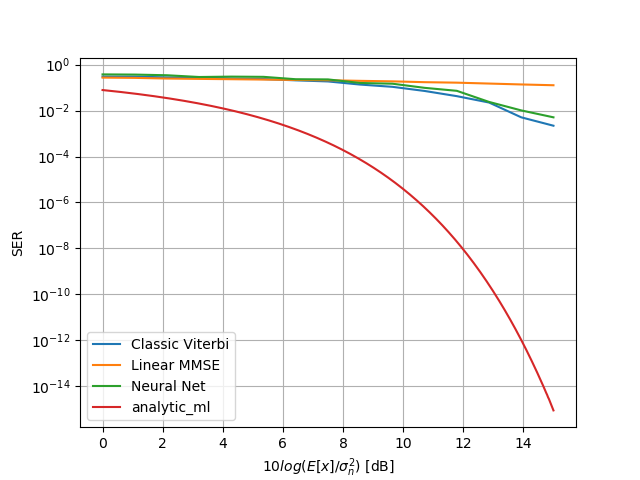
\includegraphics[width=\textwidth,height = 10cm]{results/lti_normal}
		  \caption{Detection performance over LTI channel with AWGN}
	  \label{fig:LTI performance}
\end{figure}

\subsubsection{LTI + Quantizer Channel}

To evaluate decoder performance in the non-linear channel setting, we apply a quantizer, $\text{Quant}()$, to the output of the previous LTI + AWGN channel.
\begin{equation*}
y[\text{k}] = text{Quant}(\sum_{\mathrm{l=1}}^{\mathrm{L}} a[l]x[\text{k}-l]) + n[\text{k}].
\end{equation*}
 Here we evaluate performance under two levels of quantization severity: rounding channel output down to a given number of decimal places . Figure \ref{fig:Quantized Overlay} depicts the quantizer and its impact on the received symbols from the LTI channel. The resulting performance is seen in Figure \ref{fig:Quantized performance}. Notice that this is essentially a reduction of the original channel states as there is now redundancy that was not previously present. 

\begin{figure}[H]
\centering
	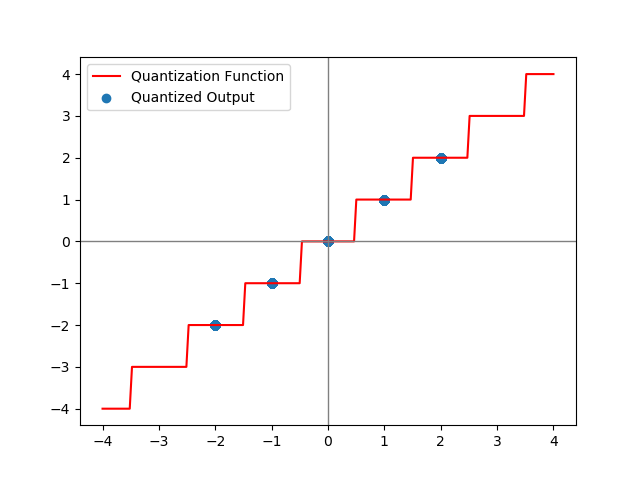
\includegraphics[width=10cm,height = 10cm]{system_model/quantizer_overlay}
			  \caption{Quantized output of LTI channel overlayed on the applied quantization function. TODO decide on axis titles }
	  \label{fig:Quantized Overlay}
\end{figure}

\begin{figure}[H]
	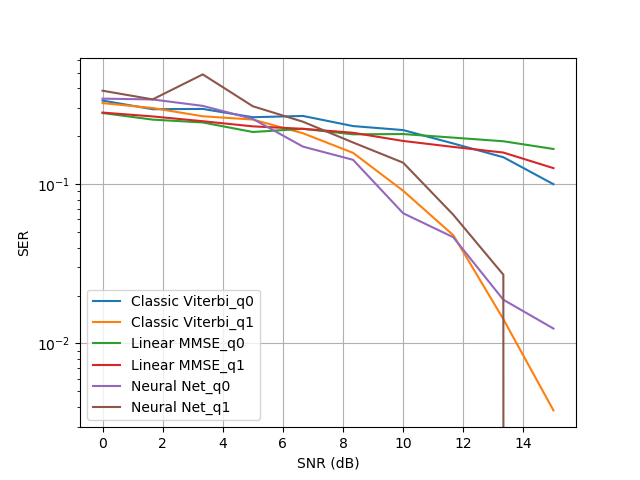
\includegraphics[width=\textwidth,height = 10cm]{results/quantized_before_noise}
		  \caption{Detection performance over LTI channel with AWGN and quantization}
	  \label{fig:Quantized performance}
\end{figure}


\subsubsection{molecular communication Channel}
Lastly, the performance of the neural network based detector is evaluated data collected from a molecular communication channel. ... Explain if there are any results to report. 

\section{Conclusion}
The proposed detection method from \cite{shlezinger2019viterbinet} is evaluated in channels for which $p(y_{\mathrm{i}}|\mathbf{x}_{\mathrm{i-L+1}}^{\mathrm{i}}),$ is unknown and non-linear. Simulation results indicate that this detector can successfully learn
$p(y_{\mathrm{i}}|\mathbf{x}_{\mathrm{i-L+1}}^{\mathrm{i}})$ for non-linear channels. A method for reducing the complexity of the resulting Viterbi Algorithm is also proposed, however the method of state reduction for the channel needs to be further investigated to improve the poor performance observed. 
\par 
In this work the MLSE is found using the Viterbi Algorithm. The same metrics can also be used in optimizing other performance metrics. In \cite{shlezinger2020datadriven} these estimate metrics have been used for minimize bit error rate estimation using the BCJR algorithm. 

Extensions of specific work: 
More on reduced state.
Using other channels and repeat online type of updates for dynamic channels for these more challenging channels. 
Learning channel changes in cases for which coherence time is shorter than updates to network made by pilot symbols. 

General method extensions:


\newpage
\bibliography{report_bib}{}
\bibliographystyle{plain}
\end{document}
